% Created by tikzDevice version 0.10.1 on 2017-10-30 17:28:47
% !TEX encoding = UTF-8 Unicode
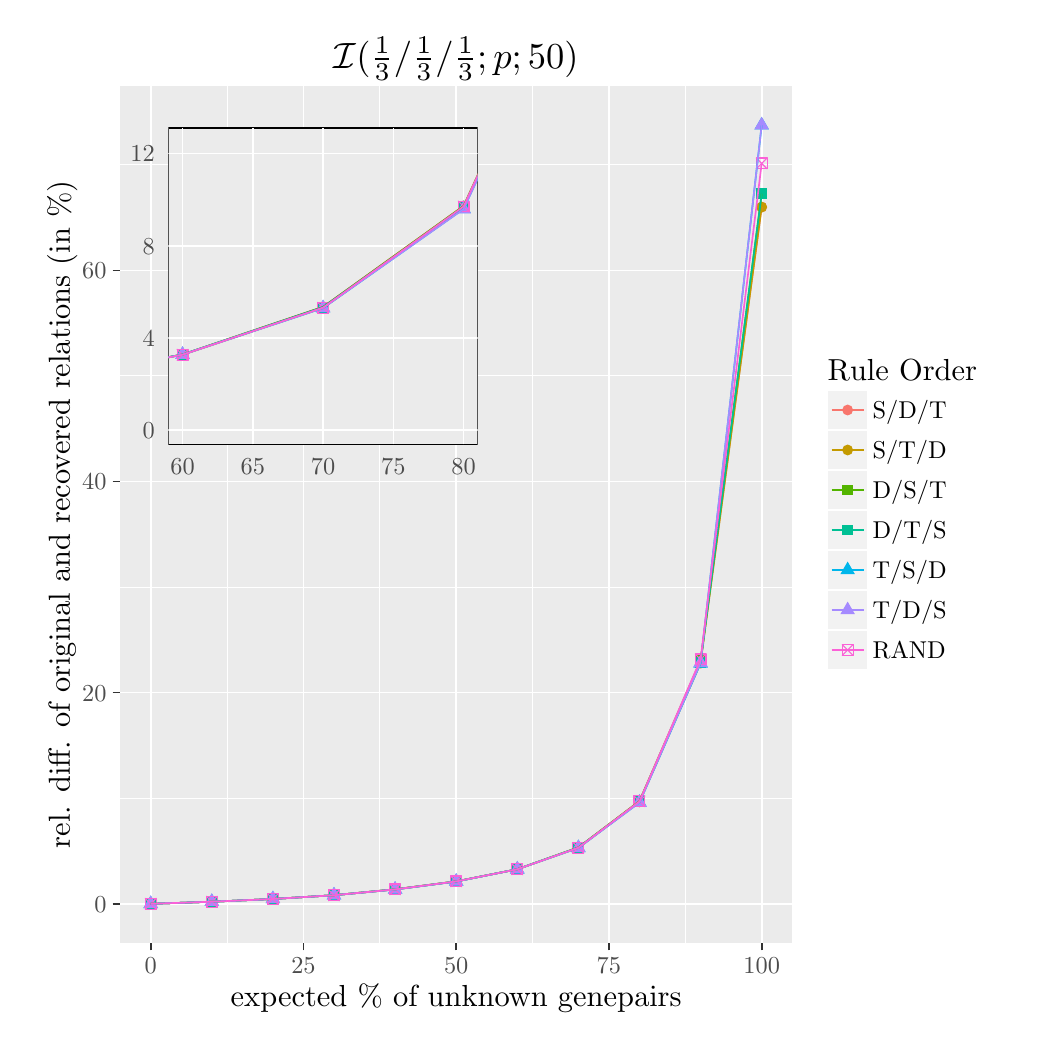
\begin{tikzpicture}[x=1pt,y=1pt]
\definecolor{fillColor}{RGB}{255,255,255}
\path[use as bounding box,fill=fillColor,fill opacity=0.00] (0,0) rectangle (361.35,361.35);
\begin{scope}
\path[clip] (  0.00,  0.00) rectangle (361.35,361.35);
\definecolor{drawColor}{RGB}{255,255,255}
\definecolor{fillColor}{RGB}{255,255,255}

\path[draw=drawColor,line width= 0.6pt,line join=round,line cap=round,fill=fillColor] (  0.00,  0.00) rectangle (361.35,361.35);
\end{scope}
\begin{scope}
\path[clip] ( 33.42, 30.69) rectangle (276.26,340.16);
\definecolor{fillColor}{gray}{0.92}

\path[fill=fillColor] ( 33.42, 30.69) rectangle (276.26,340.16);
\definecolor{drawColor}{RGB}{255,255,255}

\path[draw=drawColor,line width= 0.3pt,line join=round] ( 33.42, 82.91) --
	(276.26, 82.91);

\path[draw=drawColor,line width= 0.3pt,line join=round] ( 33.42,159.21) --
	(276.26,159.21);

\path[draw=drawColor,line width= 0.3pt,line join=round] ( 33.42,235.51) --
	(276.26,235.51);

\path[draw=drawColor,line width= 0.3pt,line join=round] ( 33.42,311.81) --
	(276.26,311.81);

\path[draw=drawColor,line width= 0.3pt,line join=round] ( 72.06, 30.69) --
	( 72.06,340.16);

\path[draw=drawColor,line width= 0.3pt,line join=round] (127.25, 30.69) --
	(127.25,340.16);

\path[draw=drawColor,line width= 0.3pt,line join=round] (182.44, 30.69) --
	(182.44,340.16);

\path[draw=drawColor,line width= 0.3pt,line join=round] (237.63, 30.69) --
	(237.63,340.16);

\path[draw=drawColor,line width= 0.6pt,line join=round] ( 33.42, 44.75) --
	(276.26, 44.75);

\path[draw=drawColor,line width= 0.6pt,line join=round] ( 33.42,121.06) --
	(276.26,121.06);

\path[draw=drawColor,line width= 0.6pt,line join=round] ( 33.42,197.36) --
	(276.26,197.36);

\path[draw=drawColor,line width= 0.6pt,line join=round] ( 33.42,273.66) --
	(276.26,273.66);

\path[draw=drawColor,line width= 0.6pt,line join=round] ( 44.46, 30.69) --
	( 44.46,340.16);

\path[draw=drawColor,line width= 0.6pt,line join=round] ( 99.65, 30.69) --
	( 99.65,340.16);

\path[draw=drawColor,line width= 0.6pt,line join=round] (154.84, 30.69) --
	(154.84,340.16);

\path[draw=drawColor,line width= 0.6pt,line join=round] (210.03, 30.69) --
	(210.03,340.16);

\path[draw=drawColor,line width= 0.6pt,line join=round] (265.23, 30.69) --
	(265.23,340.16);
\definecolor{fillColor}{RGB}{248,118,109}

\path[fill=fillColor] ( 44.46, 44.75) circle (  1.96);

\path[fill=fillColor] ( 66.54, 45.51) circle (  1.96);

\path[fill=fillColor] ( 88.61, 46.51) circle (  1.96);

\path[fill=fillColor] (110.69, 47.87) circle (  1.96);

\path[fill=fillColor] (132.77, 50.02) circle (  1.96);

\path[fill=fillColor] (154.84, 52.87) circle (  1.96);

\path[fill=fillColor] (176.92, 57.27) circle (  1.96);

\path[fill=fillColor] (199.00, 65.16) circle (  1.96);

\path[fill=fillColor] (221.07, 81.88) circle (  1.96);

\path[fill=fillColor] (243.15,132.58) circle (  1.96);

\path[fill=fillColor] (265.23,296.52) circle (  1.96);
\definecolor{fillColor}{RGB}{196,154,0}

\path[fill=fillColor] ( 44.46, 44.75) circle (  1.96);

\path[fill=fillColor] ( 66.54, 45.49) circle (  1.96);

\path[fill=fillColor] ( 88.61, 46.50) circle (  1.96);

\path[fill=fillColor] (110.69, 47.86) circle (  1.96);

\path[fill=fillColor] (132.77, 49.96) circle (  1.96);

\path[fill=fillColor] (154.84, 52.87) circle (  1.96);

\path[fill=fillColor] (176.92, 57.22) circle (  1.96);

\path[fill=fillColor] (199.00, 65.00) circle (  1.96);

\path[fill=fillColor] (221.07, 81.60) circle (  1.96);

\path[fill=fillColor] (243.15,131.75) circle (  1.96);

\path[fill=fillColor] (265.23,296.52) circle (  1.96);
\definecolor{fillColor}{RGB}{83,180,0}

\path[fill=fillColor] ( 42.50, 42.79) --
	( 46.42, 42.79) --
	( 46.42, 46.72) --
	( 42.50, 46.72) --
	cycle;

\path[fill=fillColor] ( 64.58, 43.55) --
	( 68.50, 43.55) --
	( 68.50, 47.48) --
	( 64.58, 47.48) --
	cycle;

\path[fill=fillColor] ( 86.65, 44.54) --
	( 90.58, 44.54) --
	( 90.58, 48.46) --
	( 86.65, 48.46) --
	cycle;

\path[fill=fillColor] (108.73, 45.91) --
	(112.65, 45.91) --
	(112.65, 49.83) --
	(108.73, 49.83) --
	cycle;

\path[fill=fillColor] (130.81, 48.04) --
	(134.73, 48.04) --
	(134.73, 51.97) --
	(130.81, 51.97) --
	cycle;

\path[fill=fillColor] (152.88, 50.90) --
	(156.81, 50.90) --
	(156.81, 54.82) --
	(152.88, 54.82) --
	cycle;

\path[fill=fillColor] (174.96, 55.30) --
	(178.88, 55.30) --
	(178.88, 59.23) --
	(174.96, 59.23) --
	cycle;

\path[fill=fillColor] (197.03, 63.17) --
	(200.96, 63.17) --
	(200.96, 67.10) --
	(197.03, 67.10) --
	cycle;

\path[fill=fillColor] (219.11, 79.90) --
	(223.03, 79.90) --
	(223.03, 83.82) --
	(219.11, 83.82) --
	cycle;

\path[fill=fillColor] (241.19,130.67) --
	(245.11,130.67) --
	(245.11,134.59) --
	(241.19,134.59) --
	cycle;

\path[fill=fillColor] (263.26,299.31) --
	(267.19,299.31) --
	(267.19,303.24) --
	(263.26,303.24) --
	cycle;
\definecolor{fillColor}{RGB}{0,192,148}

\path[fill=fillColor] ( 42.50, 42.79) --
	( 46.42, 42.79) --
	( 46.42, 46.72) --
	( 42.50, 46.72) --
	cycle;

\path[fill=fillColor] ( 64.58, 43.55) --
	( 68.50, 43.55) --
	( 68.50, 47.48) --
	( 64.58, 47.48) --
	cycle;

\path[fill=fillColor] ( 86.65, 44.54) --
	( 90.58, 44.54) --
	( 90.58, 48.46) --
	( 86.65, 48.46) --
	cycle;

\path[fill=fillColor] (108.73, 45.91) --
	(112.65, 45.91) --
	(112.65, 49.83) --
	(108.73, 49.83) --
	cycle;

\path[fill=fillColor] (130.81, 48.01) --
	(134.73, 48.01) --
	(134.73, 51.93) --
	(130.81, 51.93) --
	cycle;

\path[fill=fillColor] (152.88, 50.85) --
	(156.81, 50.85) --
	(156.81, 54.77) --
	(152.88, 54.77) --
	cycle;

\path[fill=fillColor] (174.96, 55.30) --
	(178.88, 55.30) --
	(178.88, 59.23) --
	(174.96, 59.23) --
	cycle;

\path[fill=fillColor] (197.03, 63.14) --
	(200.96, 63.14) --
	(200.96, 67.06) --
	(197.03, 67.06) --
	cycle;

\path[fill=fillColor] (219.11, 79.64) --
	(223.03, 79.64) --
	(223.03, 83.56) --
	(219.11, 83.56) --
	cycle;

\path[fill=fillColor] (241.19,130.12) --
	(245.11,130.12) --
	(245.11,134.05) --
	(241.19,134.05) --
	cycle;

\path[fill=fillColor] (263.26,299.31) --
	(267.19,299.31) --
	(267.19,303.24) --
	(263.26,303.24) --
	cycle;
\definecolor{fillColor}{RGB}{0,182,235}

\path[fill=fillColor] ( 44.46, 47.80) --
	( 47.10, 43.23) --
	( 41.82, 43.23) --
	cycle;

\path[fill=fillColor] ( 66.54, 48.55) --
	( 69.18, 43.97) --
	( 63.90, 43.97) --
	cycle;

\path[fill=fillColor] ( 88.61, 49.55) --
	( 91.26, 44.97) --
	( 85.97, 44.97) --
	cycle;

\path[fill=fillColor] (110.69, 50.91) --
	(113.33, 46.33) --
	(108.05, 46.33) --
	cycle;

\path[fill=fillColor] (132.77, 52.99) --
	(135.41, 48.41) --
	(130.12, 48.41) --
	cycle;

\path[fill=fillColor] (154.84, 55.87) --
	(157.49, 51.30) --
	(152.20, 51.30) --
	cycle;

\path[fill=fillColor] (176.92, 60.28) --
	(179.56, 55.70) --
	(174.28, 55.70) --
	cycle;

\path[fill=fillColor] (199.00, 68.00) --
	(201.64, 63.42) --
	(196.35, 63.42) --
	cycle;

\path[fill=fillColor] (221.07, 84.43) --
	(223.72, 79.86) --
	(218.43, 79.86) --
	cycle;

\path[fill=fillColor] (243.15,134.71) --
	(245.79,130.14) --
	(240.51,130.14) --
	cycle;

\path[fill=fillColor] (265.23,329.14) --
	(267.87,324.57) --
	(262.58,324.57) --
	cycle;
\definecolor{fillColor}{RGB}{165,138,255}

\path[fill=fillColor] ( 44.46, 47.80) --
	( 47.10, 43.23) --
	( 41.82, 43.23) --
	cycle;

\path[fill=fillColor] ( 66.54, 48.56) --
	( 69.18, 43.98) --
	( 63.90, 43.98) --
	cycle;

\path[fill=fillColor] ( 88.61, 49.55) --
	( 91.26, 44.97) --
	( 85.97, 44.97) --
	cycle;

\path[fill=fillColor] (110.69, 50.92) --
	(113.33, 46.34) --
	(108.05, 46.34) --
	cycle;

\path[fill=fillColor] (132.77, 52.98) --
	(135.41, 48.40) --
	(130.12, 48.40) --
	cycle;

\path[fill=fillColor] (154.84, 55.87) --
	(157.49, 51.29) --
	(152.20, 51.29) --
	cycle;

\path[fill=fillColor] (176.92, 60.30) --
	(179.56, 55.72) --
	(174.28, 55.72) --
	cycle;

\path[fill=fillColor] (199.00, 68.02) --
	(201.64, 63.45) --
	(196.35, 63.45) --
	cycle;

\path[fill=fillColor] (221.07, 84.40) --
	(223.72, 79.82) --
	(218.43, 79.82) --
	cycle;

\path[fill=fillColor] (243.15,134.89) --
	(245.79,130.32) --
	(240.51,130.32) --
	cycle;

\path[fill=fillColor] (265.23,329.14) --
	(267.87,324.57) --
	(262.58,324.57) --
	cycle;
\definecolor{drawColor}{RGB}{251,97,215}

\path[draw=drawColor,line width= 0.4pt,line join=round,line cap=round] ( 42.50, 42.79) rectangle ( 46.42, 46.72);

\path[draw=drawColor,line width= 0.4pt,line join=round,line cap=round] ( 42.50, 42.79) -- ( 46.42, 46.72);

\path[draw=drawColor,line width= 0.4pt,line join=round,line cap=round] ( 42.50, 46.72) -- ( 46.42, 42.79);

\path[draw=drawColor,line width= 0.4pt,line join=round,line cap=round] ( 64.58, 43.55) rectangle ( 68.50, 47.47);

\path[draw=drawColor,line width= 0.4pt,line join=round,line cap=round] ( 64.58, 43.55) -- ( 68.50, 47.47);

\path[draw=drawColor,line width= 0.4pt,line join=round,line cap=round] ( 64.58, 47.47) -- ( 68.50, 43.55);

\path[draw=drawColor,line width= 0.4pt,line join=round,line cap=round] ( 86.65, 44.53) rectangle ( 90.58, 48.46);

\path[draw=drawColor,line width= 0.4pt,line join=round,line cap=round] ( 86.65, 44.53) -- ( 90.58, 48.46);

\path[draw=drawColor,line width= 0.4pt,line join=round,line cap=round] ( 86.65, 48.46) -- ( 90.58, 44.53);

\path[draw=drawColor,line width= 0.4pt,line join=round,line cap=round] (108.73, 45.89) rectangle (112.65, 49.82);

\path[draw=drawColor,line width= 0.4pt,line join=round,line cap=round] (108.73, 45.89) -- (112.65, 49.82);

\path[draw=drawColor,line width= 0.4pt,line join=round,line cap=round] (108.73, 49.82) -- (112.65, 45.89);

\path[draw=drawColor,line width= 0.4pt,line join=round,line cap=round] (130.81, 48.00) rectangle (134.73, 51.93);

\path[draw=drawColor,line width= 0.4pt,line join=round,line cap=round] (130.81, 48.00) -- (134.73, 51.93);

\path[draw=drawColor,line width= 0.4pt,line join=round,line cap=round] (130.81, 51.93) -- (134.73, 48.00);

\path[draw=drawColor,line width= 0.4pt,line join=round,line cap=round] (152.88, 50.89) rectangle (156.81, 54.81);

\path[draw=drawColor,line width= 0.4pt,line join=round,line cap=round] (152.88, 50.89) -- (156.81, 54.81);

\path[draw=drawColor,line width= 0.4pt,line join=round,line cap=round] (152.88, 54.81) -- (156.81, 50.89);

\path[draw=drawColor,line width= 0.4pt,line join=round,line cap=round] (174.96, 55.26) rectangle (178.88, 59.18);

\path[draw=drawColor,line width= 0.4pt,line join=round,line cap=round] (174.96, 55.26) -- (178.88, 59.18);

\path[draw=drawColor,line width= 0.4pt,line join=round,line cap=round] (174.96, 59.18) -- (178.88, 55.26);

\path[draw=drawColor,line width= 0.4pt,line join=round,line cap=round] (197.03, 63.06) rectangle (200.96, 66.98);

\path[draw=drawColor,line width= 0.4pt,line join=round,line cap=round] (197.03, 63.06) -- (200.96, 66.98);

\path[draw=drawColor,line width= 0.4pt,line join=round,line cap=round] (197.03, 66.98) -- (200.96, 63.06);

\path[draw=drawColor,line width= 0.4pt,line join=round,line cap=round] (219.11, 79.81) rectangle (223.03, 83.74);

\path[draw=drawColor,line width= 0.4pt,line join=round,line cap=round] (219.11, 79.81) -- (223.03, 83.74);

\path[draw=drawColor,line width= 0.4pt,line join=round,line cap=round] (219.11, 83.74) -- (223.03, 79.81);

\path[draw=drawColor,line width= 0.4pt,line join=round,line cap=round] (241.19,131.11) rectangle (245.11,135.04);

\path[draw=drawColor,line width= 0.4pt,line join=round,line cap=round] (241.19,131.11) -- (245.11,135.04);

\path[draw=drawColor,line width= 0.4pt,line join=round,line cap=round] (241.19,135.04) -- (245.11,131.11);

\path[draw=drawColor,line width= 0.4pt,line join=round,line cap=round] (263.26,310.34) rectangle (267.19,314.27);

\path[draw=drawColor,line width= 0.4pt,line join=round,line cap=round] (263.26,310.34) -- (267.19,314.27);

\path[draw=drawColor,line width= 0.4pt,line join=round,line cap=round] (263.26,314.27) -- (267.19,310.34);
\definecolor{drawColor}{RGB}{248,118,109}

\path[draw=drawColor,line width= 0.6pt,line join=round] ( 44.46, 44.75) --
	( 66.54, 45.51) --
	( 88.61, 46.51) --
	(110.69, 47.87) --
	(132.77, 50.02) --
	(154.84, 52.87) --
	(176.92, 57.27) --
	(199.00, 65.16) --
	(221.07, 81.88) --
	(243.15,132.58) --
	(265.23,296.52);
\definecolor{drawColor}{RGB}{196,154,0}

\path[draw=drawColor,line width= 0.6pt,line join=round] ( 44.46, 44.75) --
	( 66.54, 45.49) --
	( 88.61, 46.50) --
	(110.69, 47.86) --
	(132.77, 49.96) --
	(154.84, 52.87) --
	(176.92, 57.22) --
	(199.00, 65.00) --
	(221.07, 81.60) --
	(243.15,131.75) --
	(265.23,296.52);
\definecolor{drawColor}{RGB}{83,180,0}

\path[draw=drawColor,line width= 0.6pt,line join=round] ( 44.46, 44.75) --
	( 66.54, 45.51) --
	( 88.61, 46.50) --
	(110.69, 47.87) --
	(132.77, 50.00) --
	(154.84, 52.86) --
	(176.92, 57.26) --
	(199.00, 65.14) --
	(221.07, 81.86) --
	(243.15,132.63) --
	(265.23,301.28);
\definecolor{drawColor}{RGB}{0,192,148}

\path[draw=drawColor,line width= 0.6pt,line join=round] ( 44.46, 44.75) --
	( 66.54, 45.51) --
	( 88.61, 46.50) --
	(110.69, 47.87) --
	(132.77, 49.97) --
	(154.84, 52.81) --
	(176.92, 57.27) --
	(199.00, 65.10) --
	(221.07, 81.60) --
	(243.15,132.09) --
	(265.23,301.28);
\definecolor{drawColor}{RGB}{0,182,235}

\path[draw=drawColor,line width= 0.6pt,line join=round] ( 44.46, 44.75) --
	( 66.54, 45.50) --
	( 88.61, 46.50) --
	(110.69, 47.86) --
	(132.77, 49.94) --
	(154.84, 52.82) --
	(176.92, 57.23) --
	(199.00, 64.95) --
	(221.07, 81.38) --
	(243.15,131.66) --
	(265.23,326.09);
\definecolor{drawColor}{RGB}{165,138,255}

\path[draw=drawColor,line width= 0.6pt,line join=round] ( 44.46, 44.75) --
	( 66.54, 45.50) --
	( 88.61, 46.49) --
	(110.69, 47.86) --
	(132.77, 49.93) --
	(154.84, 52.82) --
	(176.92, 57.25) --
	(199.00, 64.97) --
	(221.07, 81.35) --
	(243.15,131.84) --
	(265.23,326.09);
\definecolor{drawColor}{RGB}{251,97,215}

\path[draw=drawColor,line width= 0.6pt,line join=round] ( 44.46, 44.75) --
	( 66.54, 45.51) --
	( 88.61, 46.50) --
	(110.69, 47.86) --
	(132.77, 49.97) --
	(154.84, 52.85) --
	(176.92, 57.22) --
	(199.00, 65.02) --
	(221.07, 81.77) --
	(243.15,133.08) --
	(265.23,312.30);
\end{scope}
\begin{scope}
\path[clip] (  0.00,  0.00) rectangle (361.35,361.35);
\definecolor{drawColor}{gray}{0.30}

\node[text=drawColor,anchor=base east,inner sep=0pt, outer sep=0pt, scale=  0.88] at ( 28.47, 41.72) {0};

\node[text=drawColor,anchor=base east,inner sep=0pt, outer sep=0pt, scale=  0.88] at ( 28.47,118.03) {20};

\node[text=drawColor,anchor=base east,inner sep=0pt, outer sep=0pt, scale=  0.88] at ( 28.47,194.33) {40};

\node[text=drawColor,anchor=base east,inner sep=0pt, outer sep=0pt, scale=  0.88] at ( 28.47,270.63) {60};
\end{scope}
\begin{scope}
\path[clip] (  0.00,  0.00) rectangle (361.35,361.35);
\definecolor{drawColor}{gray}{0.20}

\path[draw=drawColor,line width= 0.6pt,line join=round] ( 30.67, 44.75) --
	( 33.42, 44.75);

\path[draw=drawColor,line width= 0.6pt,line join=round] ( 30.67,121.06) --
	( 33.42,121.06);

\path[draw=drawColor,line width= 0.6pt,line join=round] ( 30.67,197.36) --
	( 33.42,197.36);

\path[draw=drawColor,line width= 0.6pt,line join=round] ( 30.67,273.66) --
	( 33.42,273.66);
\end{scope}
\begin{scope}
\path[clip] (  0.00,  0.00) rectangle (361.35,361.35);
\definecolor{drawColor}{gray}{0.20}

\path[draw=drawColor,line width= 0.6pt,line join=round] ( 44.46, 27.94) --
	( 44.46, 30.69);

\path[draw=drawColor,line width= 0.6pt,line join=round] ( 99.65, 27.94) --
	( 99.65, 30.69);

\path[draw=drawColor,line width= 0.6pt,line join=round] (154.84, 27.94) --
	(154.84, 30.69);

\path[draw=drawColor,line width= 0.6pt,line join=round] (210.03, 27.94) --
	(210.03, 30.69);

\path[draw=drawColor,line width= 0.6pt,line join=round] (265.23, 27.94) --
	(265.23, 30.69);
\end{scope}
\begin{scope}
\path[clip] (  0.00,  0.00) rectangle (361.35,361.35);
\definecolor{drawColor}{gray}{0.30}

\node[text=drawColor,anchor=base,inner sep=0pt, outer sep=0pt, scale=  0.88] at ( 44.46, 19.68) {0};

\node[text=drawColor,anchor=base,inner sep=0pt, outer sep=0pt, scale=  0.88] at ( 99.65, 19.68) {25};

\node[text=drawColor,anchor=base,inner sep=0pt, outer sep=0pt, scale=  0.88] at (154.84, 19.68) {50};

\node[text=drawColor,anchor=base,inner sep=0pt, outer sep=0pt, scale=  0.88] at (210.03, 19.68) {75};

\node[text=drawColor,anchor=base,inner sep=0pt, outer sep=0pt, scale=  0.88] at (265.23, 19.68) {100};
\end{scope}
\begin{scope}
\path[clip] (  0.00,  0.00) rectangle (361.35,361.35);
\definecolor{drawColor}{RGB}{0,0,0}

\node[text=drawColor,anchor=base,inner sep=0pt, outer sep=0pt, scale=  1.10] at (154.84,  7.70) {expected \% of unknown genepairs};
\end{scope}
\begin{scope}
\path[clip] (  0.00,  0.00) rectangle (361.35,361.35);
\definecolor{drawColor}{RGB}{0,0,0}

\node[text=drawColor,rotate= 90.00,anchor=base,inner sep=0pt, outer sep=0pt, scale=  1.10] at ( 15.28,185.42) {rel. diff. of original and recovered relations (in \%)};
\end{scope}
\begin{scope}
\path[clip] (  0.00,  0.00) rectangle (361.35,361.35);
\definecolor{fillColor}{RGB}{255,255,255}

\path[fill=fillColor] (284.80,124.97) rectangle (347.31,245.87);
\end{scope}
\begin{scope}
\path[clip] (  0.00,  0.00) rectangle (361.35,361.35);
\definecolor{drawColor}{RGB}{0,0,0}

\node[text=drawColor,anchor=base west,inner sep=0pt, outer sep=0pt, scale=  1.10] at (289.07,234.03) {Rule Order};
\end{scope}
\begin{scope}
\path[clip] (  0.00,  0.00) rectangle (361.35,361.35);
\definecolor{drawColor}{RGB}{255,255,255}
\definecolor{fillColor}{gray}{0.95}

\path[draw=drawColor,line width= 0.6pt,line join=round,line cap=round,fill=fillColor] (289.07,215.96) rectangle (303.52,230.42);
\end{scope}
\begin{scope}
\path[clip] (  0.00,  0.00) rectangle (361.35,361.35);
\definecolor{fillColor}{RGB}{248,118,109}

\path[fill=fillColor] (296.29,223.19) circle (  1.96);
\end{scope}
\begin{scope}
\path[clip] (  0.00,  0.00) rectangle (361.35,361.35);
\definecolor{drawColor}{RGB}{248,118,109}

\path[draw=drawColor,line width= 0.6pt,line join=round] (290.51,223.19) -- (302.08,223.19);
\end{scope}
\begin{scope}
\path[clip] (  0.00,  0.00) rectangle (361.35,361.35);
\definecolor{drawColor}{RGB}{255,255,255}
\definecolor{fillColor}{gray}{0.95}

\path[draw=drawColor,line width= 0.6pt,line join=round,line cap=round,fill=fillColor] (289.07,201.51) rectangle (303.52,215.96);
\end{scope}
\begin{scope}
\path[clip] (  0.00,  0.00) rectangle (361.35,361.35);
\definecolor{fillColor}{RGB}{196,154,0}

\path[fill=fillColor] (296.29,208.74) circle (  1.96);
\end{scope}
\begin{scope}
\path[clip] (  0.00,  0.00) rectangle (361.35,361.35);
\definecolor{drawColor}{RGB}{196,154,0}

\path[draw=drawColor,line width= 0.6pt,line join=round] (290.51,208.74) -- (302.08,208.74);
\end{scope}
\begin{scope}
\path[clip] (  0.00,  0.00) rectangle (361.35,361.35);
\definecolor{drawColor}{RGB}{255,255,255}
\definecolor{fillColor}{gray}{0.95}

\path[draw=drawColor,line width= 0.6pt,line join=round,line cap=round,fill=fillColor] (289.07,187.06) rectangle (303.52,201.51);
\end{scope}
\begin{scope}
\path[clip] (  0.00,  0.00) rectangle (361.35,361.35);
\definecolor{fillColor}{RGB}{83,180,0}

\path[fill=fillColor] (294.33,192.32) --
	(298.26,192.32) --
	(298.26,196.24) --
	(294.33,196.24) --
	cycle;
\end{scope}
\begin{scope}
\path[clip] (  0.00,  0.00) rectangle (361.35,361.35);
\definecolor{drawColor}{RGB}{83,180,0}

\path[draw=drawColor,line width= 0.6pt,line join=round] (290.51,194.28) -- (302.08,194.28);
\end{scope}
\begin{scope}
\path[clip] (  0.00,  0.00) rectangle (361.35,361.35);
\definecolor{drawColor}{RGB}{255,255,255}
\definecolor{fillColor}{gray}{0.95}

\path[draw=drawColor,line width= 0.6pt,line join=round,line cap=round,fill=fillColor] (289.07,172.60) rectangle (303.52,187.06);
\end{scope}
\begin{scope}
\path[clip] (  0.00,  0.00) rectangle (361.35,361.35);
\definecolor{fillColor}{RGB}{0,192,148}

\path[fill=fillColor] (294.33,177.87) --
	(298.26,177.87) --
	(298.26,181.79) --
	(294.33,181.79) --
	cycle;
\end{scope}
\begin{scope}
\path[clip] (  0.00,  0.00) rectangle (361.35,361.35);
\definecolor{drawColor}{RGB}{0,192,148}

\path[draw=drawColor,line width= 0.6pt,line join=round] (290.51,179.83) -- (302.08,179.83);
\end{scope}
\begin{scope}
\path[clip] (  0.00,  0.00) rectangle (361.35,361.35);
\definecolor{drawColor}{RGB}{255,255,255}
\definecolor{fillColor}{gray}{0.95}

\path[draw=drawColor,line width= 0.6pt,line join=round,line cap=round,fill=fillColor] (289.07,158.15) rectangle (303.52,172.60);
\end{scope}
\begin{scope}
\path[clip] (  0.00,  0.00) rectangle (361.35,361.35);
\definecolor{fillColor}{RGB}{0,182,235}

\path[fill=fillColor] (296.29,168.43) --
	(298.94,163.85) --
	(293.65,163.85) --
	cycle;
\end{scope}
\begin{scope}
\path[clip] (  0.00,  0.00) rectangle (361.35,361.35);
\definecolor{drawColor}{RGB}{0,182,235}

\path[draw=drawColor,line width= 0.6pt,line join=round] (290.51,165.37) -- (302.08,165.37);
\end{scope}
\begin{scope}
\path[clip] (  0.00,  0.00) rectangle (361.35,361.35);
\definecolor{drawColor}{RGB}{255,255,255}
\definecolor{fillColor}{gray}{0.95}

\path[draw=drawColor,line width= 0.6pt,line join=round,line cap=round,fill=fillColor] (289.07,143.69) rectangle (303.52,158.15);
\end{scope}
\begin{scope}
\path[clip] (  0.00,  0.00) rectangle (361.35,361.35);
\definecolor{fillColor}{RGB}{165,138,255}

\path[fill=fillColor] (296.29,153.97) --
	(298.94,149.39) --
	(293.65,149.39) --
	cycle;
\end{scope}
\begin{scope}
\path[clip] (  0.00,  0.00) rectangle (361.35,361.35);
\definecolor{drawColor}{RGB}{165,138,255}

\path[draw=drawColor,line width= 0.6pt,line join=round] (290.51,150.92) -- (302.08,150.92);
\end{scope}
\begin{scope}
\path[clip] (  0.00,  0.00) rectangle (361.35,361.35);
\definecolor{drawColor}{RGB}{255,255,255}
\definecolor{fillColor}{gray}{0.95}

\path[draw=drawColor,line width= 0.6pt,line join=round,line cap=round,fill=fillColor] (289.07,129.24) rectangle (303.52,143.69);
\end{scope}
\begin{scope}
\path[clip] (  0.00,  0.00) rectangle (361.35,361.35);
\definecolor{drawColor}{RGB}{251,97,215}

\path[draw=drawColor,line width= 0.4pt,line join=round,line cap=round] (294.33,134.50) rectangle (298.26,138.43);

\path[draw=drawColor,line width= 0.4pt,line join=round,line cap=round] (294.33,134.50) -- (298.26,138.43);

\path[draw=drawColor,line width= 0.4pt,line join=round,line cap=round] (294.33,138.43) -- (298.26,134.50);
\end{scope}
\begin{scope}
\path[clip] (  0.00,  0.00) rectangle (361.35,361.35);
\definecolor{drawColor}{RGB}{251,97,215}

\path[draw=drawColor,line width= 0.6pt,line join=round] (290.51,136.47) -- (302.08,136.47);
\end{scope}
\begin{scope}
\path[clip] (  0.00,  0.00) rectangle (361.35,361.35);
\definecolor{drawColor}{RGB}{0,0,0}

\node[text=drawColor,anchor=base west,inner sep=0pt, outer sep=0pt, scale=  0.88] at (305.33,220.16) {S/D/T};
\end{scope}
\begin{scope}
\path[clip] (  0.00,  0.00) rectangle (361.35,361.35);
\definecolor{drawColor}{RGB}{0,0,0}

\node[text=drawColor,anchor=base west,inner sep=0pt, outer sep=0pt, scale=  0.88] at (305.33,205.71) {S/T/D};
\end{scope}
\begin{scope}
\path[clip] (  0.00,  0.00) rectangle (361.35,361.35);
\definecolor{drawColor}{RGB}{0,0,0}

\node[text=drawColor,anchor=base west,inner sep=0pt, outer sep=0pt, scale=  0.88] at (305.33,191.25) {D/S/T};
\end{scope}
\begin{scope}
\path[clip] (  0.00,  0.00) rectangle (361.35,361.35);
\definecolor{drawColor}{RGB}{0,0,0}

\node[text=drawColor,anchor=base west,inner sep=0pt, outer sep=0pt, scale=  0.88] at (305.33,176.80) {D/T/S};
\end{scope}
\begin{scope}
\path[clip] (  0.00,  0.00) rectangle (361.35,361.35);
\definecolor{drawColor}{RGB}{0,0,0}

\node[text=drawColor,anchor=base west,inner sep=0pt, outer sep=0pt, scale=  0.88] at (305.33,162.34) {T/S/D};
\end{scope}
\begin{scope}
\path[clip] (  0.00,  0.00) rectangle (361.35,361.35);
\definecolor{drawColor}{RGB}{0,0,0}

\node[text=drawColor,anchor=base west,inner sep=0pt, outer sep=0pt, scale=  0.88] at (305.33,147.89) {T/D/S};
\end{scope}
\begin{scope}
\path[clip] (  0.00,  0.00) rectangle (361.35,361.35);
\definecolor{drawColor}{RGB}{0,0,0}

\node[text=drawColor,anchor=base west,inner sep=0pt, outer sep=0pt, scale=  0.88] at (305.33,133.44) {RAND};
\end{scope}
\begin{scope}
\path[clip] (  0.00,  0.00) rectangle (361.35,361.35);
\definecolor{drawColor}{RGB}{0,0,0}

\node[text=drawColor,anchor=base,inner sep=0pt, outer sep=0pt, scale=  1.32] at (154.84,346.76) {$\mathcal{I}(\frac{1}{3}/\frac{1}{3}/\frac{1}{3};p;50)$};
\end{scope}
\begin{scope}
\path[clip] ( 54.20,216.81) rectangle (162.61,325.21);
\definecolor{drawColor}{RGB}{255,255,255}
\definecolor{fillColor}{RGB}{255,255,255}

\path[draw=drawColor,line width= 0.6pt,line join=round,line cap=round,fill=fillColor] ( 54.20,216.81) rectangle (162.61,325.21);
\end{scope}
\begin{scope}
\path[clip] ( 50.88,210.75) rectangle (162.61,325.21);
\definecolor{drawColor}{RGB}{0,0,0}
\definecolor{fillColor}{gray}{0.92}

\path[draw=drawColor,line width= 0.6pt,line join=round,line cap=round,fill=fillColor] ( 50.88,210.75) rectangle (162.61,325.21);
\definecolor{drawColor}{RGB}{255,255,255}

\path[draw=drawColor,line width= 0.6pt,line join=round] ( 50.88,215.95) --
	(162.61,215.95);

\path[draw=drawColor,line width= 0.6pt,line join=round] ( 50.88,249.25) --
	(162.61,249.25);

\path[draw=drawColor,line width= 0.6pt,line join=round] ( 50.88,282.55) --
	(162.61,282.55);

\path[draw=drawColor,line width= 0.6pt,line join=round] ( 50.88,315.85) --
	(162.61,315.85);

\path[draw=drawColor,line width= 0.6pt,line join=round] ( 55.96,210.75) --
	( 55.96,325.21);

\path[draw=drawColor,line width= 0.6pt,line join=round] ( 81.35,210.75) --
	( 81.35,325.21);

\path[draw=drawColor,line width= 0.6pt,line join=round] (106.74,210.75) --
	(106.74,325.21);

\path[draw=drawColor,line width= 0.6pt,line join=round] (132.14,210.75) --
	(132.14,325.21);

\path[draw=drawColor,line width= 0.6pt,line join=round] (157.53,210.75) --
	(157.53,325.21);
\definecolor{fillColor}{RGB}{248,118,109}

\path[fill=fillColor] (  5.17,233.66) circle (  1.96);

\path[fill=fillColor] ( 55.96,243.27) circle (  1.96);

\path[fill=fillColor] (106.74,260.48) circle (  1.96);

\path[fill=fillColor] (157.53,296.96) circle (  1.96);
\definecolor{fillColor}{RGB}{196,154,0}

\path[fill=fillColor] (  5.17,233.65) circle (  1.96);

\path[fill=fillColor] ( 55.96,243.16) circle (  1.96);

\path[fill=fillColor] (106.74,260.12) circle (  1.96);

\path[fill=fillColor] (157.53,296.35) circle (  1.96);
\definecolor{fillColor}{RGB}{83,180,0}

\path[fill=fillColor] (  3.21,231.68) --
	(  7.13,231.68) --
	(  7.13,235.60) --
	(  3.21,235.60) --
	cycle;

\path[fill=fillColor] ( 54.00,241.29) --
	( 57.92,241.29) --
	( 57.92,245.21) --
	( 54.00,245.21) --
	cycle;

\path[fill=fillColor] (104.78,258.46) --
	(108.71,258.46) --
	(108.71,262.39) --
	(104.78,262.39) --
	cycle;

\path[fill=fillColor] (155.57,294.96) --
	(159.49,294.96) --
	(159.49,298.88) --
	(155.57,298.88) --
	cycle;
\definecolor{fillColor}{RGB}{0,192,148}

\path[fill=fillColor] (  3.21,231.56) --
	(  7.13,231.56) --
	(  7.13,235.49) --
	(  3.21,235.49) --
	cycle;

\path[fill=fillColor] ( 54.00,241.29) --
	( 57.92,241.29) --
	( 57.92,245.22) --
	( 54.00,245.22) --
	cycle;

\path[fill=fillColor] (104.78,258.39) --
	(108.71,258.39) --
	(108.71,262.31) --
	(104.78,262.31) --
	cycle;

\path[fill=fillColor] (155.57,294.40) --
	(159.49,294.40) --
	(159.49,298.32) --
	(155.57,298.32) --
	cycle;
\definecolor{fillColor}{RGB}{0,182,235}

\path[fill=fillColor] (  5.17,236.61) --
	(  7.81,232.03) --
	(  2.53,232.03) --
	cycle;

\path[fill=fillColor] ( 55.96,246.23) --
	( 58.60,241.65) --
	( 53.31,241.65) --
	cycle;

\path[fill=fillColor] (106.74,263.06) --
	(109.39,258.49) --
	(104.10,258.49) --
	cycle;

\path[fill=fillColor] (157.53,298.93) --
	(160.17,294.35) --
	(154.89,294.35) --
	cycle;
\definecolor{fillColor}{RGB}{165,138,255}

\path[fill=fillColor] (  5.17,236.60) --
	(  7.81,232.02) --
	(  2.53,232.02) --
	cycle;

\path[fill=fillColor] ( 55.96,246.27) --
	( 58.60,241.69) --
	( 53.31,241.69) --
	cycle;

\path[fill=fillColor] (106.74,263.12) --
	(109.39,258.54) --
	(104.10,258.54) --
	cycle;

\path[fill=fillColor] (157.53,298.85) --
	(160.17,294.27) --
	(154.89,294.27) --
	cycle;
\definecolor{drawColor}{RGB}{251,97,215}

\path[draw=drawColor,line width= 0.4pt,line join=round,line cap=round] (  3.21,231.65) rectangle (  7.13,235.58);

\path[draw=drawColor,line width= 0.4pt,line join=round,line cap=round] (  3.21,231.65) -- (  7.13,235.58);

\path[draw=drawColor,line width= 0.4pt,line join=round,line cap=round] (  3.21,235.58) -- (  7.13,231.65);

\path[draw=drawColor,line width= 0.4pt,line join=round,line cap=round] ( 54.00,241.19) rectangle ( 57.92,245.11);

\path[draw=drawColor,line width= 0.4pt,line join=round,line cap=round] ( 54.00,241.19) -- ( 57.92,245.11);

\path[draw=drawColor,line width= 0.4pt,line join=round,line cap=round] ( 54.00,245.11) -- ( 57.92,241.19);

\path[draw=drawColor,line width= 0.4pt,line join=round,line cap=round] (104.78,258.21) rectangle (108.71,262.13);

\path[draw=drawColor,line width= 0.4pt,line join=round,line cap=round] (104.78,258.21) -- (108.71,262.13);

\path[draw=drawColor,line width= 0.4pt,line join=round,line cap=round] (104.78,262.13) -- (108.71,258.21);

\path[draw=drawColor,line width= 0.4pt,line join=round,line cap=round] (155.57,294.77) rectangle (159.49,298.69);

\path[draw=drawColor,line width= 0.4pt,line join=round,line cap=round] (155.57,294.77) -- (159.49,298.69);

\path[draw=drawColor,line width= 0.4pt,line join=round,line cap=round] (155.57,298.69) -- (159.49,294.77);
\definecolor{drawColor}{RGB}{248,118,109}

\path[draw=drawColor,line width= 0.6pt,line join=round] (  0.00,233.02) --
	(  5.17,233.66) --
	( 55.96,243.27) --
	(106.74,260.48) --
	(157.53,296.96) --
	(187.09,361.35);
\definecolor{drawColor}{RGB}{196,154,0}

\path[draw=drawColor,line width= 0.6pt,line join=round] (  0.00,233.01) --
	(  5.17,233.65) --
	( 55.96,243.16) --
	(106.74,260.12) --
	(157.53,296.35) --
	(187.69,361.35);
\definecolor{drawColor}{RGB}{83,180,0}

\path[draw=drawColor,line width= 0.6pt,line join=round] (  0.00,233.01) --
	(  5.17,233.64) --
	( 55.96,243.25) --
	(106.74,260.43) --
	(157.53,296.92) --
	(187.07,361.35);
\definecolor{drawColor}{RGB}{0,192,148}

\path[draw=drawColor,line width= 0.6pt,line join=round] (  0.00,232.90) --
	(  5.17,233.53) --
	( 55.96,243.26) --
	(106.74,260.35) --
	(157.53,296.36) --
	(187.49,361.35);
\definecolor{drawColor}{RGB}{0,182,235}

\path[draw=drawColor,line width= 0.6pt,line join=round] (  0.00,232.92) --
	(  5.17,233.56) --
	( 55.96,243.18) --
	(106.74,260.01) --
	(157.53,295.88) --
	(187.84,361.35);
\definecolor{drawColor}{RGB}{165,138,255}

\path[draw=drawColor,line width= 0.6pt,line join=round] (  0.00,232.91) --
	(  5.17,233.55) --
	( 55.96,243.22) --
	(106.74,260.07) --
	(157.53,295.80) --
	(187.74,361.35);
\definecolor{drawColor}{RGB}{251,97,215}

\path[draw=drawColor,line width= 0.6pt,line join=round] (  0.00,232.97) --
	(  5.17,233.61) --
	( 55.96,243.15) --
	(106.74,260.17) --
	(157.53,296.73) --
	(186.84,361.35);
\end{scope}
\begin{scope}
\path[clip] (  0.00,  0.00) rectangle (361.35,361.35);
\definecolor{drawColor}{gray}{0.30}

\node[text=drawColor,anchor=base east,inner sep=0pt, outer sep=0pt, scale=  0.88] at ( 45.93,212.92) {0};

\node[text=drawColor,anchor=base east,inner sep=0pt, outer sep=0pt, scale=  0.88] at ( 45.93,246.22) {4};

\node[text=drawColor,anchor=base east,inner sep=0pt, outer sep=0pt, scale=  0.88] at ( 45.93,279.52) {8};

\node[text=drawColor,anchor=base east,inner sep=0pt, outer sep=0pt, scale=  0.88] at ( 45.93,312.82) {12};
\end{scope}
\begin{scope}
\path[clip] (  0.00,  0.00) rectangle (361.35,361.35);
\definecolor{drawColor}{gray}{0.30}

\node[text=drawColor,anchor=base,inner sep=0pt, outer sep=0pt, scale=  0.88] at ( 55.96,199.74) {60};

\node[text=drawColor,anchor=base,inner sep=0pt, outer sep=0pt, scale=  0.88] at ( 81.35,199.74) {65};

\node[text=drawColor,anchor=base,inner sep=0pt, outer sep=0pt, scale=  0.88] at (106.74,199.74) {70};

\node[text=drawColor,anchor=base,inner sep=0pt, outer sep=0pt, scale=  0.88] at (132.14,199.74) {75};

\node[text=drawColor,anchor=base,inner sep=0pt, outer sep=0pt, scale=  0.88] at (157.53,199.74) {80};
\end{scope}
\end{tikzpicture}
